\section{Symbolic Execution in Presence of Unbounded Loops\label{sec-motor-control}}

Many programs targeting REDFIN share the distinctive feature of
the energy estimation program considered in section~\S\ref{sec-verification},
i.e. the existence of an  \emph{upper bound on execution time},
since their termination does not depend on input data.
However, other programs may have a loop
which is guarded by a termination condition that involves computation
considering the input parameters of the program, thus making the loop
\emph{unbounded}.

Presence of unbounded loops makes program verification by symbolic execution considerably
harder~\cite[p.~50:20]{SurveySymExec-CSUR18}, since the number of program execution
paths becomes infinite. In this section we consider an example
of control program that drives a stepper motor and verify one of its essential
safety properties by formulating it as a~\emph{loop invariant} and ensuring that the
invariant holds for every possible state of the loop.

\subsection{Stepper Motor Control Program}

Stepper motors are often deployed as parts of antenna and solar panel pointing units
in space satellites. We consider a program for controlling a motor with
one degree of freedom. The control algorithm~\ref{alg-motor} expects three input
parameters:
\begin{itemize}
\item $dist$ --- the distance to move the motor
\item $v_{max}$ --- the maximal permitted velocity
\item $a_{max}$ --- the maximal permitted acceleration
\end{itemize}

\noindent
and computes a series of
displacement and velocity values that will be used to move the motor. Since the algorithm is
designed for controlling a stepper motor, the calculations happen in~\emph{discreet time},
i.e. every iteration of the $while$ loop corresponds to a time interval; thus
the deceleration (i.e. braking) distance is computed as
$s_{decel} = a_{max} \cdot \frac{decel\_steps \cdot (decel\_steps + 1)}{2}$, where
$decel\_steps = \frac{v}{a_{max}}$ is the number of decelerating iterations
needed for a full stop. The conditional statement on starting in line 9 decides whether
to accelerate, to keep the velocity or to decelerate;
see Fig.~\ref{fig-motor} for example plots of velocity and distance travelled
against time. The spike on the bottom-left of the velocity graph illustrates
the edge covered by the conditional statement on line 18: if the velocity is zero, but the target
distance has not yet been reached, the motor must be moved further.

\begin{algorithm}[h]
  \begin{algorithmic}[1]
\Require {$dist$, $v_{max}$, $a_{max}$}
\State $s \gets 0$
\State $v \gets 0$
\While {$true$}
  % Compute deceleration distance based on current speed
  \State $decel\_steps\gets v / a_{max}$
  \algorithmiccomment{Compute deceleration distance based on current velocity}
  \State $s_{decel} \gets a_{max} \cdot decel\_steps \cdot (decel\_steps + 1) / 2$
  \If {$decel\_steps \cdot a_{max} \neq v$}
    \State $s_{decel} \gets s_{decel} + v$
  \EndIf
  \State {$v_{next} = min(v_{max}, dist, v + a_{max})$}
  \If {$s + s_{decel} + v_{next} \leq dist$}
    \State $v \gets v_{next}$ \algorithmiccomment{accelerate}
  \ElsIf {$s + s_{decel} + v \leq dist$}
    \State $ v \gets v $     \algorithmiccomment{keep velocity}
  \Else
     \algorithmiccomment{decelerate}
    \If {$v > decel\_steps \cdot a_{max}$}
      \State $v \gets decel\_steps \cdot a_{max}$
    \Else
      \State $v \gets v - a_{max}$
      \EndIf
  \EndIf
  \If {$v = 0$}
    \If {$s \neq dist$}  \algorithmiccomment{accelerate again to reach target}
      % didn't quite reach our target after deceleration
      % => accelerate again
      \State $v \gets min(dist - s, a_{max})$
    \Else
      % reached target
      \State $break$  \algorithmiccomment{terminate execution}
      \EndIf
      \EndIf
  \State $s \gets s + v$
\EndWhile
\end{algorithmic}
\caption{Motor Control Algorithm\label{alg-motor}}
\end{algorithm}
\begin{figure}[h]
  \centerline{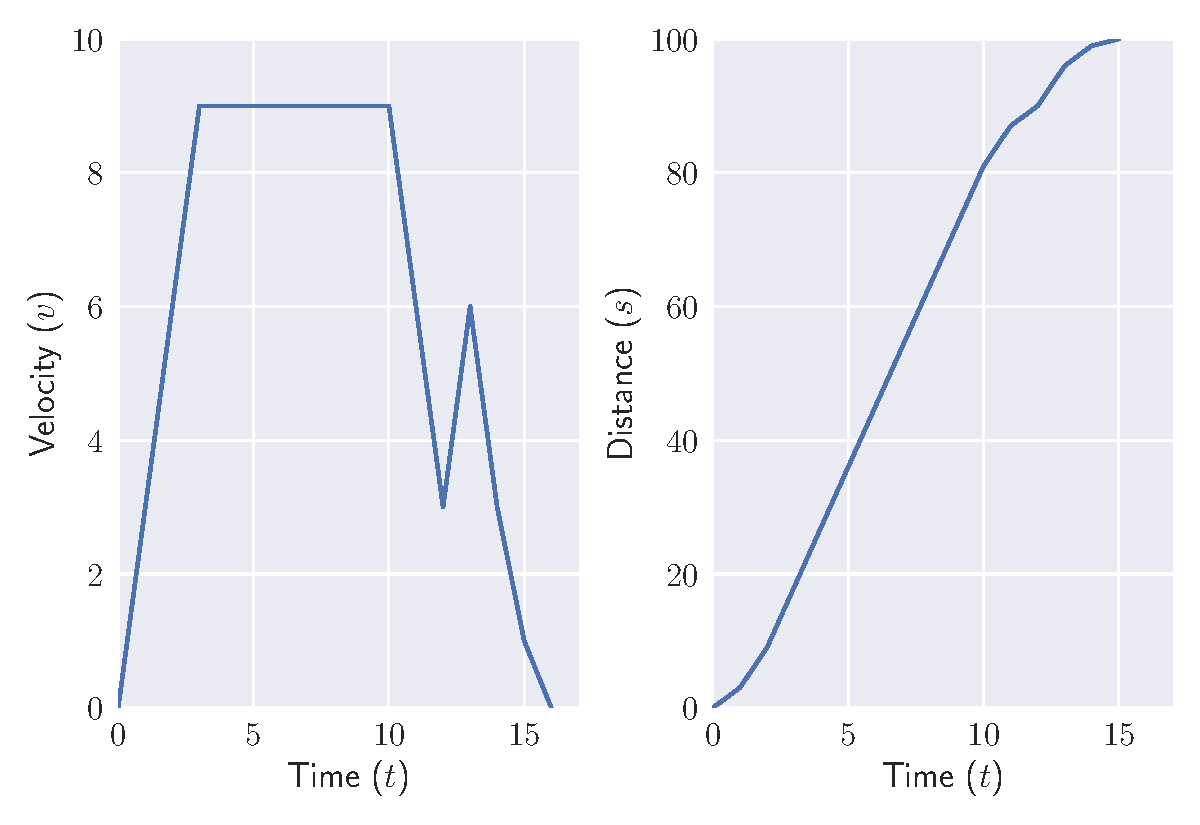
\includegraphics[scale=0.65]{fig/motor_control_graph.pdf}}
  % \vspace{-13mm}
\caption{Velocity ($v$) and distance travelled ($s$) plotted against time ($t$)\label{fig-motor}}
\Description[Please consult the text of this section for the description]{}
\end{figure}

To be deployed into REDFIN, the Algorithm~\ref{alg-motor} has been manually
implemented in REDFIN assembly. The resulting assembly program comprises 85 lines of
assembly and closely mirrors the high-level pseudocode. As a sample, consider a fragment of
the program's symbolic execution tree that corresponds to the decision whether to
accelerate, keep velocity or decelerate the motor (Fig.~\ref{fig-sym-tree}).

\begin{figure}[h]
\centerline{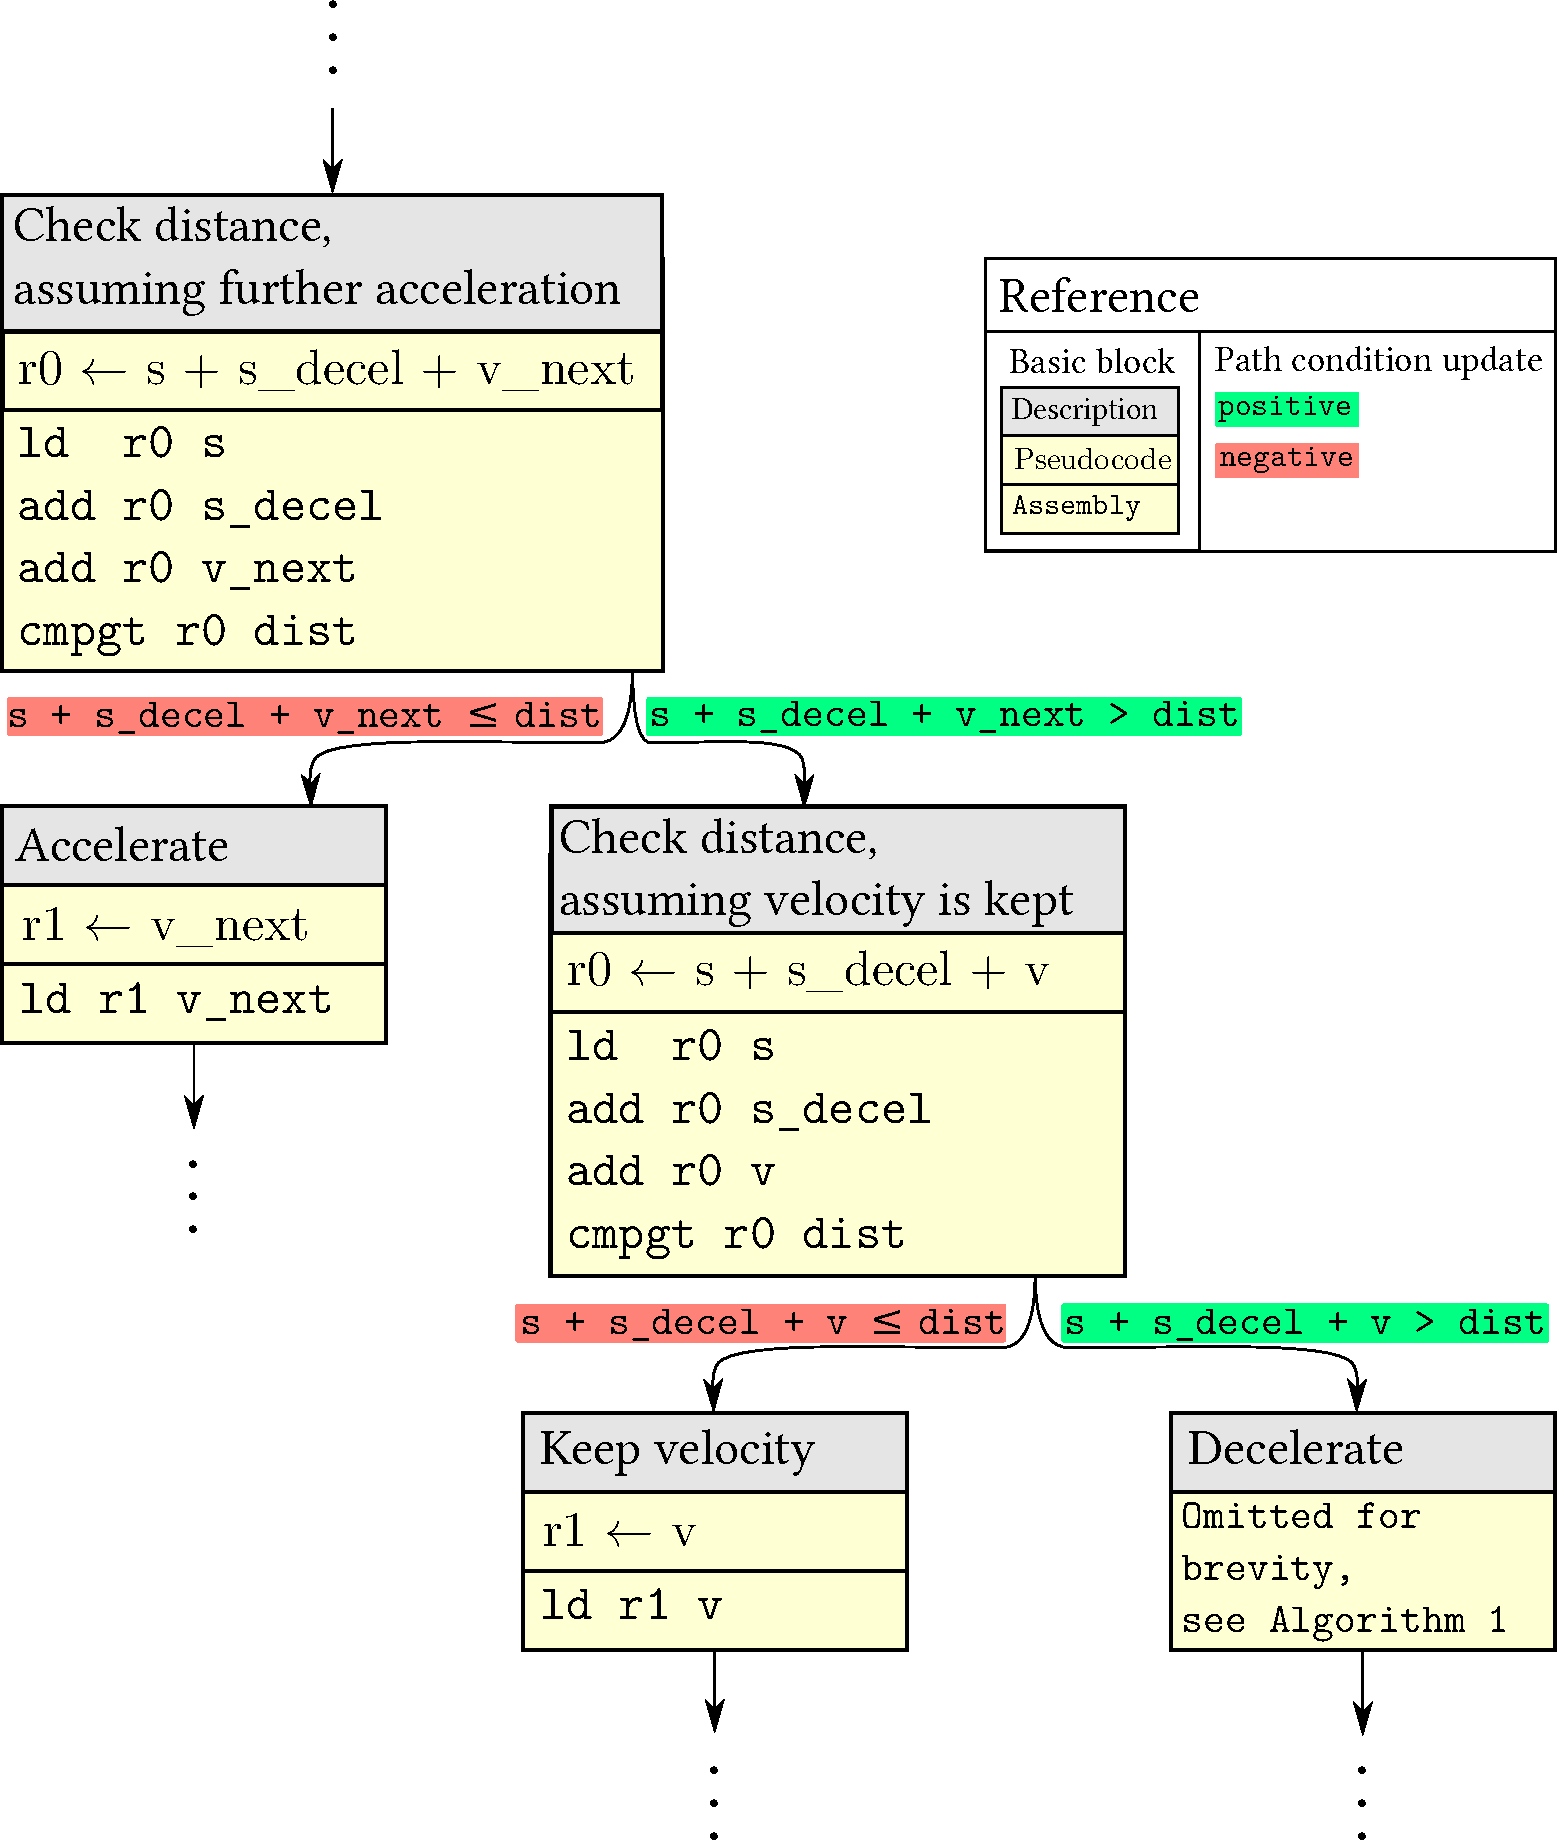
\includegraphics[scale=0.4]{fig/sym-tree.pdf}}
\caption{Symbolic execution tree of a code fragment with conditional branching\label{fig-sym-tree}}
\Description[Please consult the text of this section for the description]{}
\end{figure}

The decision is based on first estimating the resulting distance travelled using
the next potential value $v_{next}$ as velocity and if $dist$ is not covered by that
the motor will be accelerated; otherwise the resulting distance gets estimated
using the current velocity $v$ and in case $v$ is sufficient it will be kept as the
velocity; otherwise the motor will be decelerated. These changes of velocity in
a simulation on concrete data are illustrated by Fig.~\ref{fig-motor} (left).

\subsection{Loop Invariant Verification}

In order to ensure that the motor will not introduce disturbances
and will not lead the whole unit out of its normal mode of operation, the velocity and
acceleration of the motor must be kept in safe limits. This verification condition
is motivated by the correctness requirements of the whole space satellite unit.

More formally, the verification condition means
that at any iteration $t$ of the loop the values of the
expressions $v^t$, velocity, and $\left| v^t_{next} - v^t \right|$,
acceleration, must never exceed the parameters $v_{max}$ and $a_{max}$, respectively.
This property is the loop invariant for the motor control program which
ensures that velocity and acceleration always stay within their safe bounds. We
formalise it as the following predicate that universally quantifies over the
program's inputs and the loop's state:

\begin{figure}[H]
\vspace{-4mm}
\begin{tcolorbox}
\LARGE{
\[
  \forall\ v_{max}\ a_{max}\ t\ v^t\ v^t_{next},\ v^t \leq v_{max} \land \left| v^t_{next} - v^t \right| \leq a_{max}
\]}
\end{tcolorbox}
\vspace{-3mm}
\caption{Motor control loop invariant\label{fig-loop-invariant}}
\vspace{-3mm}
\end{figure}

\noindent
We will verify the loop invariant by using the verification framework in
\emph{branching} mode~\S\ref{sec-transformer}. While symbolic execution with
merging, which is implemented by the framework's \emph{merging} mode, allows
for intuitive formulation of properties for whole-program verification and
is very useful for verifying finite programs, as we have
reported in the section~\S\ref{sec-verification}, in presence of branches guarded
by symbolic values it suffers from \emph{symbolic non-termination}; thus,
for verifying the loop invariant, we rely on branching symbolic execution.

\noindent
We take the following generic approach:

\begin{itemize}
  \item Obtain the binary tree-shaped trace by symbolic execution in~\emph{branching} mode
  \item Split the trace into linear paths, thus enumerating all the possible
    execution scenarios
  \item For every path perform the analysis:
    \begin{enumerate}
      \item Extract the relevant parts of the state from the~\emph{last} node in
        the path, i.e. symbolic expressions stored representing $s$,
        $v$ and $v_{next}$
      \item Extract the terminal~\emph{path condition} $\phi$
            from the~\emph{last} node in the path
      \item Construct a symbolic expression representing the~\emph{verification condition},
            $\psi$, i.e. the one in Fig.~\ref{fig-loop-invariant}
      \item To verify the property in the given path by checking the following
        formula for satisfiability: $\phi \land \lnot\psi$, i.e. the path condition
        conjoined with negated verification condition

    \end{enumerate}
    \item  The property holds if and only if for every path the solver returns
           \emph{unsat}, i.e. there are no assignments of the variables which
           satisfy the~\emph{negation} of the property to check, considering the
           terminal path condition.
\end{itemize}

As illustrated by Fig.~\ref{fig-sym-tree}, every conditional jump instruction produces
two branches in the symbolic execution tree: the one
where the current path condition is conjoined with the jump's guard and the one where it is
conjoined with the guard's negation. However, if the resulting
conjunction is unsatisfiable, the corresponding branch need not to be explored
and can be safely pruned.
Thus the symbolic execution engine need to call an SMT solver every
time a conditional jump is encountered to check if the path conditions of the branches
are satisfiable.

Checking satisfiability of execution path is essential for mitigation of the path explosion
problem. Precondition, when available, is assigned as the initial path condition and thus
will become a subterm of every formula submitted to the solver.
Identifying correct preconditions is essential for verification since they may
drastically reduce the number of satisfiable paths in the symbolic execution tree
of the program that is being verified.

With the branch pruning optimisation in place and the parameters restricted
to $dist \in \mathopen[1, 200\mathclose]$, $v_{max} \in \mathopen[1, 30\mathclose]$ and
$a_{max} \in \mathopen[1, 30\mathclose]$ the verification of the loop invariant
takes around 40 minutes on a conventional workstation\footnote{We use a laptop
with 2.90GHz Intel Core i5-4300U processor, 8GB RAM (3MB cache),
and the SMT solver Z3 version 4.5.1 (64-bit).}.